
\documentclass[journal,12pt,twocolumn]{article}
\usepackage{graphicx}
\usepackage[none]{hyphenat}
\usepackage[margin=0.5in]{geometry}
\usepackage[cmex10]{amsmath}
\usepackage{array}
\usepackage{booktabs}
\usepackage{gensymb}
\usepackage{textcomp}
\title{\textbf{Conic Assignment}}
\author{Manideep Parusha - FWC22004}
\date{\today}

\providecommand{\norm}[1]{\left\lVert#1\right\rVert}
\providecommand{\abs}[1]{\left\vert#1\right\vert}
\let\vec\mathbf
\newcommand{\myvec}[1]{\ensuremath{\begin{pmatrix}#1\end{pmatrix}}}
\newcommand{\mydet}[1]{\ensuremath{\begin{vmatrix}#1\end{vmatrix}}}
\providecommand{\brak}[1]{\ensuremath{\left(#1\right)}}
\let\vec\mathbf
\begin{document}

\maketitle
\section*{Problem}
\paragraph{Find the equation of the circle with center (2,2) and passes through the point (4,5).}

\section*{Solution}

\begin{figure}[h]
\centering
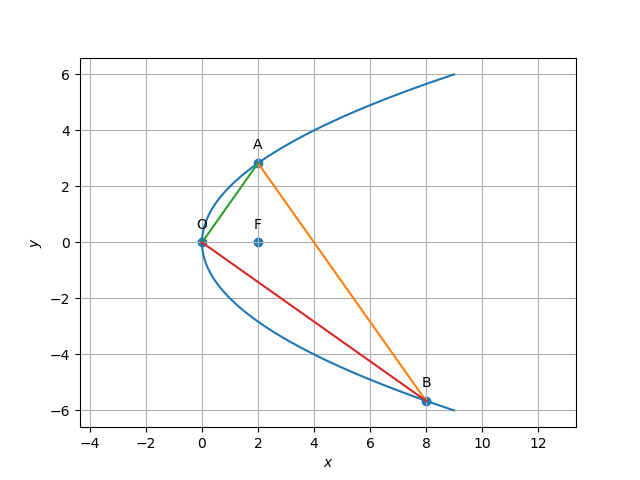
\includegraphics[width=\columnwidth]{figs/plot_con.png}
	\caption{Circle with center (2,2) and passing through (4,5)}
\label{fig:con_py}
\end{figure}

\subsection*{Construction}
Input taken for the construction of the circle are it's center and point it is passing through.

\begin{table}[h]
	\centering
\setlength\extrarowheight{2pt}
	\begin{tabular}{|c|c|c|}
		\hline
		\textbf{Symbol} & \textbf{Value} & \textbf{Description} \\
		\hline
		C & (2,2) & circle center\\
		\hline
		A & (4,5) & point on circle\\
		\hline
		r & $\norm{A-C}$ & circle radius\\
		\hline
	\end{tabular}
\end{table}
Let us assume a circle with radius 'r' and center at $\boldsymbol{C}$ which is passing through a point $\boldsymbol{A}$.\\
Radius of the circle is the distance between center and any point on circle.
\begin{align}
	r = \norm{A-C}\\
	r = \sqrt{13}
\end{align}

The desired circle can be expressed as a conic with the parameters
\begin{align}
	\vec{V} = \vec{I} \\
	\vec{u}= \myvec{-2 & -2} 
\end{align}
the constant 'f' in the equation can be calculated as
\begin{align}
	f = \norm{\vec{C}}^2 - \vec{r}^2 \\
	f = \sqrt{2^2 + 2^2}^2 - 13 \\
	f = -5
\end{align}

The general equation of the circle as a conic is
\begin{equation}
	\vec{x}^T\vec{V}\vec{x} + 2\vec{u}^T\vec{x} + f = 0
\end{equation}
by subtitution the considered parameters in the general form, 
\begin{equation}
	\vec{x}^T\vec{x} + 2\myvec{-2&-2}\vec{x} - 5 = 0
	\label{eqn:circle}
\end{equation}
this the desired equation of the circle with center at (2,2) and passes through (4,5).\\
We can verify the equation by substituting the point in the equation,

\begin{align}
	\vec{x} = \myvec{4 & 5}
\end{align}
from the eqn \ref{eqn:circle}
\begin{align}
	\myvec{4 & 5} \myvec{4\\5} + 2\myvec{-2\\-2}\myvec{4&5} -5 = 0\\
	\implies
	4^2 + 5 ^2 -16 -20 -5 =0 \\
	\implies
	0=0\\
	LHS = RHS
\end{align}
Hence, equation \ref{eqn:circle} is the required circle equation.






\end{document}
